\begin{figure}[ht]
\centering
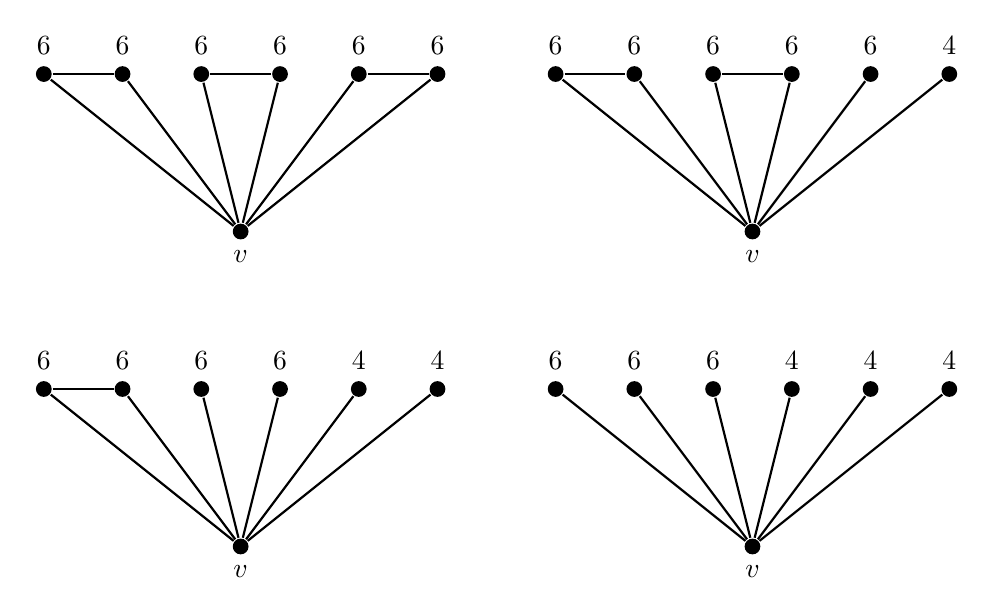
\begin{tikzpicture}[
       thick,
       acteur/.style={
         circle,
         fill=black,
         thick,
         inner sep=2pt,
         minimum size=0.2cm
       }
     ]

       \node (v) at (-3.5,0) [acteur,label=below:$v$]{};
       \node (w1) at (-6,2)[acteur,label=above:$6$]{}; 
       \node (w2) at (-5,2) [acteur,label=above:$6$]{}; 
       \node (w3) at (-4,2) [acteur,label=above:$6$]{};
       \node (w4) at (-3,2) [acteur,label=above:$6$]{};
       \node (w5) at (-2,2) [acteur,label=above:$6$]{};
       \node (w6) at (-1,2) [acteur,label=above:$6$]{};
  
       \draw (v) -- (w1);
       \draw (v) -- (w2);
       \draw (v) -- (w3);
       \draw (v) -- (w4);
       \draw (v) -- (w5);
       \draw (v) -- (w6);
       
       \draw (w1) -- (w2);
       \draw (w3) -- (w4);
       \draw (w5) -- (w6);
       
       
       \node (v) at (3,0) [acteur,label=below:$v$]{};
       \node (w1) at (0.5,2)[acteur,label=above:$6$]{}; 
       \node (w2) at (1.5,2) [acteur,label=above:$6$]{}; 
       \node (w3) at (2.5,2) [acteur,label=above:$6$]{};
       \node (w4) at (3.5,2) [acteur,label=above:$6$]{};
       \node (w5) at (4.5,2) [acteur,label=above:$6$]{};
       \node (w6) at (5.5,2) [acteur,label=above:$4$]{};
  
       \draw (v) -- (w1);
       \draw (v) -- (w2);
       \draw (v) -- (w3);
       \draw (v) -- (w4);
       \draw (v) -- (w5);
       \draw (v) -- (w6);
       
       \draw (w1) -- (w2);
       \draw (w3) -- (w4);
       
       
       \node (v) at (-3.5,-4) [acteur,label=below:$v$]{};
       \node (w1) at (-6,-2)[acteur,label=above:$6$]{}; 
       \node (w2) at (-5,-2) [acteur,label=above:$6$]{}; 
       \node (w3) at (-4,-2) [acteur,label=above:$6$]{};
       \node (w4) at (-3,-2) [acteur,label=above:$6$]{};
       \node (w5) at (-2,-2) [acteur,label=above:$4$]{};
       \node (w6) at (-1,-2) [acteur,label=above:$4$]{};
  
       \draw (v) -- (w1);
       \draw (v) -- (w2);
       \draw (v) -- (w3);
       \draw (v) -- (w4);
       \draw (v) -- (w5);
       \draw (v) -- (w6);
       
       \draw (w1) -- (w2);
    
       
       \node (v) at (3,-4) [acteur,label=below:$v$]{};
       \node (w1) at (0.5,-2)[acteur,label=above:$6$]{}; 
       \node (w2) at (1.5,-2) [acteur,label=above:$6$]{}; 
       \node (w3) at (2.5,-2) [acteur,label=above:$6$]{};
       \node (w4) at (3.5,-2) [acteur,label=above:$4$]{};
       \node (w5) at (4.5,-2) [acteur,label=above:$4$]{};
       \node (w6) at (5.5,-2) [acteur,label=above:$4$]{};
  
       \draw (v) -- (w1);
       \draw (v) -- (w2);
       \draw (v) -- (w3);
       \draw (v) -- (w4);
       \draw (v) -- (w5);
       \draw (v) -- (w6);
       

\end{tikzpicture}
  \caption{Possible shapes of $A_v$ if $\deg_G(v)=6$}
  \label{figure8:Figure 8}
\end{figure}
